\section{Generator} \label{sec: generator}

The \textbf{Generator} can execute five actions: conversion from image to map, map generation, map labelling, map augmentation and map modification.

\textbf{Conversion.} An image can be converted into an internal \textbf{Map} and saved into the maps directory from \textbf{Resources}. The image can be a software drawn image or Simultaneous Localization and Mapping (SLAM) image \cite{dissanayake2001solution} output from a real robot, as long as it follows the conventions imposed by the image converter: an agent represented by a true red circle has to be present, a goal represented by a true green circle has to be present and the obstacles need to be in the grey-black colour range (See Figure \ref{fig: converted map}).

\begin{figure}[h]
  \centering
  \begin{subfigure}[b]{0.3\linewidth}
    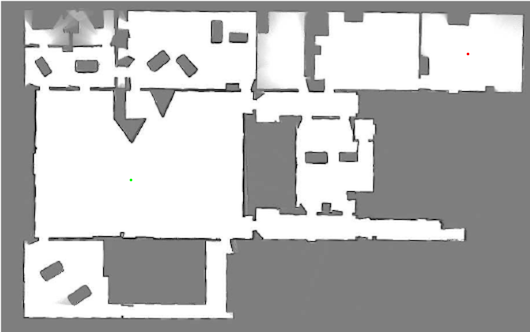
\includegraphics[width=\linewidth]{images/map10.png}
     \caption{Original SLAM Image}
  \end{subfigure}
  \hspace{1.5cm}
  \begin{subfigure}[b]{0.3\linewidth}
    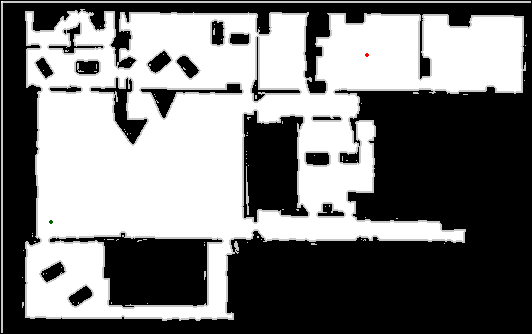
\includegraphics[width=\linewidth]{images/screenshot_108.png}
     \caption{Converted \textbf{Map}}
  \end{subfigure}
  \caption{Example of the conversion process from the \textbf{Generator}}
  \label{fig: converted map}
\end{figure}

%\todo{Sajad: do you ever refer to Fig 4.2-h? it seeme like a  repetition of 4.3-b.}
% The repetion is used to hilight that the simulator has a grid display as well, even if it is the same algorithm

%\todo{Sajad: It is very common to use 'Figure X' instead of 'figure X' and 'Algorithm Y' instead of 'Algorithm Y' and 'Table Z' instead of 'table Z' when you want to refer a figure, alg, or table in the text.}

% comment messes latex will put at top

\textbf{Generation.} The generation procedure accepts as input, different hyper-parameters such as the type of generated map, number of generated maps, obstacle fill rate range, number of obstacle range, minimum room size range and maximum room size range, which define the structure of the maps. When a range is given as input, the generator picks a random number between the range and feeds it into the associated map type generator. Currently, the generator can produce three types of maps: uniform random fill map (See Algorithm \ref{alg: Uniform random fill generator}), block map (See Algorithm \ref{alg: Block map generator}) and house map (See Algorithm \ref{alg: House generator}) (See Figure \ref{fig: generated maps}) and it can easily be extended to support different synthetic maps such as mazes and cave generation using cellular automata. All generated maps are placed into a new \textbf{Atlas} directory which is a custom directory that saves files using the index number. It keeps track of the next available index, and thus, when a new file is saved, it is "appended" to it. \textbf{Atlas} directories are used for easier indexing operations such as index loading and index saving (the file system service is described in Appendix \ref{sec: infra}).

\begin{figure}[h!]
  \centering
  \begin{subfigure}[b]{0.3\linewidth}
    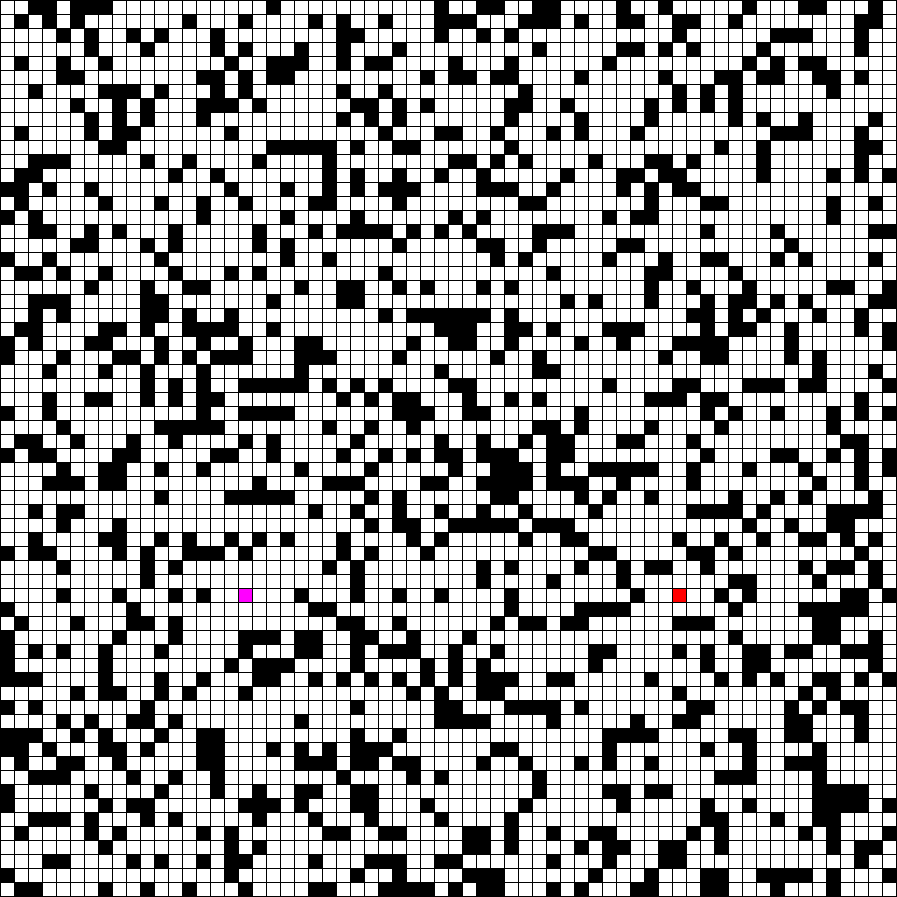
\includegraphics[width=\linewidth]{images/screenshot_52.png}
     \caption{Uniform random fill (64x64 dimension, [0.1, 0.3] obstacle fill rate range)\newline}
  \end{subfigure}
  \hfill
  \begin{subfigure}[b]{0.3\linewidth}
    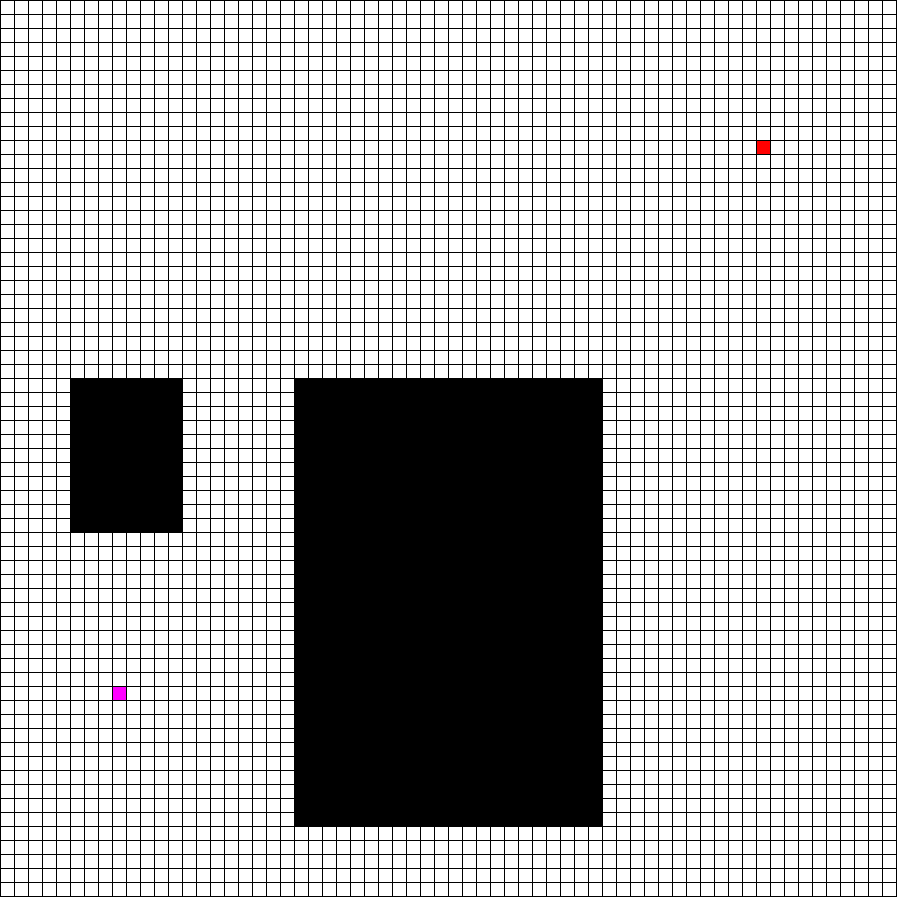
\includegraphics[width=\linewidth]{images/screenshot_54.png}
     \caption{Block map (64x64 dimension, [0.1, 0.3] obstacle fill rate range, [1, 6] number of obstacles range)}
  \end{subfigure}
  \hfill
  \begin{subfigure}[b]{0.3\linewidth}
    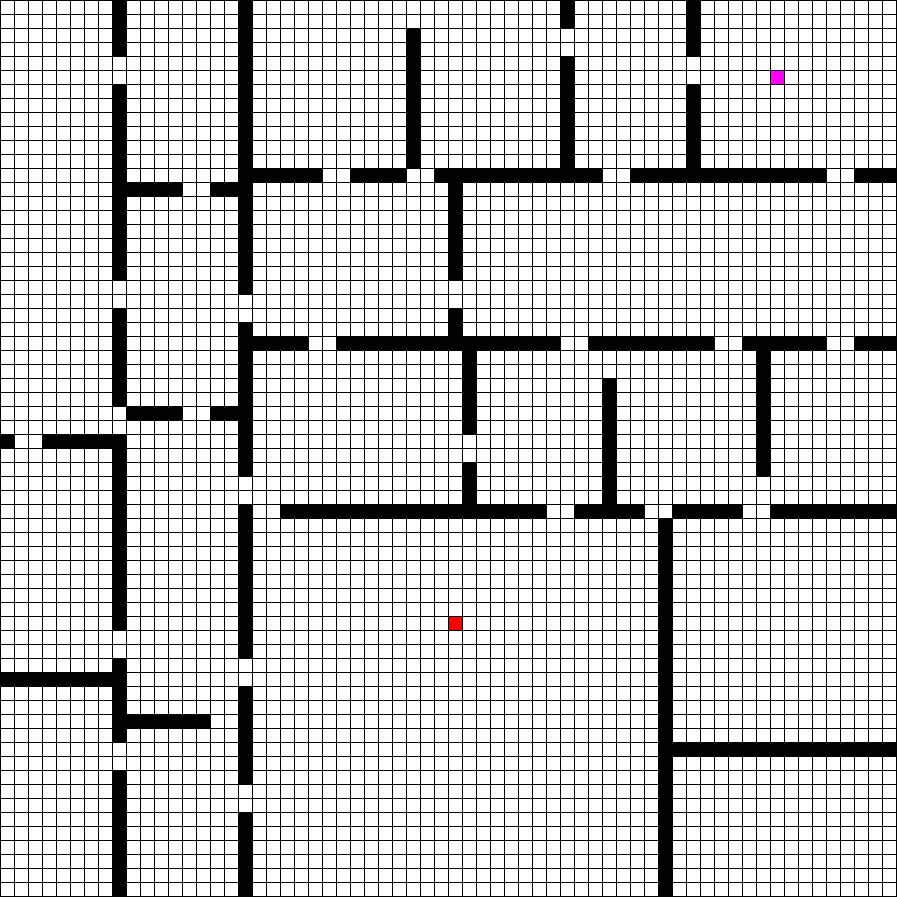
\includegraphics[width=\linewidth]{images/screenshot_53.png}
     \caption{House (64x64 dimension, [8, 15] minimum room size range, [35, 45] maximum room size range)}
  \end{subfigure}
  \caption{The current generated maps are: (a) Uniform random fill (10000 samples), (b) Block map (10000 samples), (c) House atlas (10000 samples). We will use magenta colour for the goal for all generated maps as the dark green goal is quite hard to spot}
  \label{fig: generated maps}
\end{figure}

\begin{algorithm}[!htb]
\caption{Uniform random fill generator}
\label{alg: Uniform random fill generator}
\begin{algorithmic}[1]
\Procedure{Generate-Uniform-Random-Fill-Map}{$dimension$, $obstacle\_fill\_rate$}
    \State Initialise empty $map$ of dimension $dimension$
    \State $fill \gets obstacle\_fill\_rate * dimension.width * dimension.height$
    \State $nr\_of\_obstacles \gets 0$
    \State
    \While {$nr\_of\_obstacles < fill$}
        \State $obstacle\_position \gets$ random position within $dimension$
        \If {$obstacle\_position$ is free on $map$}
            \State place unity obstacle at $obstacle\_position$ on $map$
            \State increment $nr\_of\_obstacles$ 
        \EndIf
    \EndWhile
    \State
    \State place agent and goal at random free positions on $map$
    \State \Return $map$
\EndProcedure
\end{algorithmic}
\end{algorithm}

\begin{algorithm}[!htb]
\caption{Block map generator}
\label{alg: Block map generator}
\begin{algorithmic}[1]
\Procedure{Generate-Block-Map}{$dimension$, $obstacle\_fill\_rate$, $nr\_of\_obstacles$}
    \State Initialise empty $map$ of dimension $dimension$
    \State $fill \gets obstacle\_fill\_rate * dimension.width * dimension.height$
    \State
    \For {$i$ in [0, $nr\_of\_obstacles$)}
        \State $next\_obst\_fill \gets$ random value from $fill$
        \While {can't place block}
            \State $first\_side \gets$ random value from $next\_obst\_fill$
            \State $second\_side \gets$ $next\_obst\_fill$ / $first\_side$
            \State try to place block of dimension ($first\_side$, $second\_side$) on random position (blocks may overlap)
        \EndWhile
        \State 
        \State $fill \gets fill - next\_obst\_fill$
    \EndFor
    \State
    \State place agent and goal at random free positions on $map$
    \State \Return $map$
\EndProcedure
\end{algorithmic}
\end{algorithm}

\begin{algorithm}[!htb]
\caption{House generator}
\label{alg: House generator}
\begin{algorithmic}[1]

\Procedure{Subdivide}{$top\_left\_corner, dimension$}
    \If{can't split anymore due to $min\_room\_size$}
        \State place a room at $top\_left\_corner$ with dimension $dimension$
    \EndIf
    \State
    \If{$dimension \leq max\_room\_size$}
        \State 50\% change to place a room at $top\_left\_corner$ with dimension $dimension$
    \EndIf
    \State
    \State random pick vertical or horizontal
    \State random split vertical/horizontal into 2 blocks: $first\_block$, $second\_block$
    \State
    \State $\textit{Subdivide}(first\_block\_top\_left\_corner, first\_block\_dimension)$
    \State $\textit{Subdivide}(second\_block\_top\_left\_corner, second\_block\_dimension)$
\EndProcedure

\Procedure{Generate-House-Map}{$dimension$, $min\_room\_size$, $max\_room\_size$}
    \State Initialise empty $map$ of dimension $dimension$
    \State
    \State $\textit{Subdivide}((-1, -1), dimension + 1)$
    \For{\ \textbf{each} $room$}
        \State get $room$ walls and add doors with probability 25\% (max 1 door per wall)
    \EndFor
    \State
    \State place agent and goal at random free positions on $map$
    \State \Return $map$
\EndProcedure
\end{algorithmic}
\end{algorithm}

\clearpage

\textbf{Labelling.} The labelling procedure takes a map \textbf{Atlas} and converts it into training data by picking only the specified features and labels. The training data is then saved as a \texttt{.pickle} file with name format as \texttt{training\_\{atlas name\}\_\{number of samples\}}. The structure of the training data is based on normal \textit{python} objects (\texttt{List[Dict[str, Any]]}) for quick inspection and analysis. Features/labels are picked by using the \textbf{MapProcessing} component (See Table \ref{tab: gen_label_list} for feature reference). A* is used as ground truth for feature/label generation. All features/labels can be saved as a variable sequence (needed for LSTM) or single global input (needed for auto-encoder).

\begin{table}[h!]
    \centerfloat
    \begin{tabular}{|M{5cm}|M{9cm}|}
        \hline
        \textbf{Feature/Label Key} &  \textbf{Description} \\
        \hline
        agent\_position & The current agent position \\
        \hline
        direction\_to\_goal & The current direction from the agent to the goal \\
        \hline
        direction\_to\_goal\_normalized & The normalised direction from the agent to the goal \\
        \hline
        distance\_to\_goal & The current Euclidean distance from the agent to the goal\\
        \hline
        distance\_to\_goal\_normalized(n) & The current normalised Euclidean distance from the agent to the goal (normalisation is done by clamping the output between [0, n))\\
        \hline
        raycast\_8 & The current distance from agent to obstacles on all eight directions (vertical, horizontal, diagonal) \\
        \hline
        raycast\_8\_normalized(n) & The current normalised distance from agent to obstacles on all eight directions (vertical, horizontal, diagonal) (normalisation is done by clamping the output between [0, n)) \\
        \hline
        agent\_goal\_angle & The current angle defined by the line segment from the agent to the goal (code $torch.atan2(v.y, v.x)$, where $v$ is the line segment)\\
        \hline
        valid\_moves & The current 0-1 tensor which describes in which direction (vertical, horizontal, diagonal) is agent movement available (1 is available) \\
        \hline
        global\_map & The current whole map obstacles given as a normalised 0-1 tensor (1 is obstacle)\\
        \hline
        local\_map & Like global\_map, but it has $9\times9$ dimension and agent is centred \\
        \hline
        next\_position & The next move direction that the agent should take \\
        \hline
        next\_position\_index & The next action that the agent should take given as an index from 0 to 7 \\
        \hline
    \end{tabular}
    \caption{\textbf{Generator} list of features and labels. A* is used as ground truth for label annotation}
    \label{tab: gen_label_list}
\end{table}

\textbf{Augmentation.} The augmentation procedure takes an existing training data file and augments it with the specified extra features and labels. It is used to remove the need for re-generating a whole training set.

\textbf{Modification.} A custom lambda function which takes as input a \textbf{Map} and returns another \textbf{Map} can be defined to modify the underlining structure of the map (e.g. modify the agent position, the goal position, create doors, etc.).